\section{Introduction}


\subsection{Motivation and Relevance of Anomaly Detection in Electric Vehicle Supply Equipment (EVSE)}

Electric Vehicle Supply Equipment (EVSE) has gained significant importance in recent years \cite{paper_relevance_EVSE}. Analyzing the market sales of electric vehicles (EVs), we observe a remarkable growth: in 2012, only 120,000 EVs were sold, whereas by 2021, sales had surged to nearly 6.6 million. And to achieve net-zero CO2 emissions by 2050, as planed by the European Union \cite{EU2050}, the number of EVs must continue to rise substantially—requiring an 11-fold increase from current levels by 2030 alone \cite{Number_of_EVSE_sales}.\\
To manage the much higher demand for EVs on our roads, we can assume that the market for EVSE will grow similarly to the resale of EVs. The correlation between the number of EVs and the number of EVSE is high. If we analyze the reasale from the last few years, we can see that the top five countries in the European Union like Germany, Netherlands, France, and Belgium with the best EVSE infrastructure are also the top five with the largest market share of EVs \cite{ladeinfrastruktur}.
\begin{figure}[htbp]
  \centering
  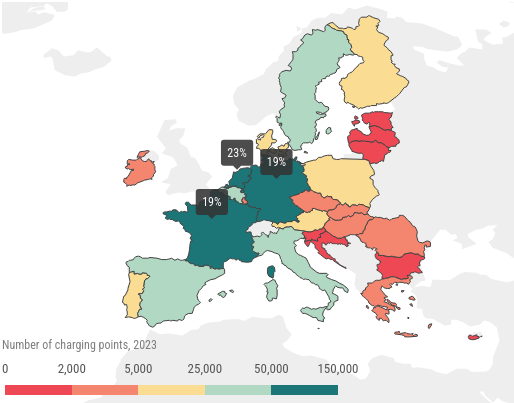
\includegraphics[width=0.5\textwidth]{pics/chargingPointsInfrastructure.png}
  \caption{Availability of public charging points and market share of electric cars in the EU\cite{ladeinfrastruktur}.}
  \label{fig:chargingPointsInfrastructure}
\end{figure}
\\
With the growing number of EVSE, particularly Charging Stations (CS), the interest of cybercriminal groups in attacking these systems is also increasing. At first glance, EVSE systems may not appear to be direct targets for accessing critical data or manipulation. However, they can serve as entry points to gain access to more sensitive or private information \cite{nature2025}. The following figure illustrates how EVSE components, such as charging stations, can act as access nodes to critical or private data.
\begin{figure}[H]
  \centering
  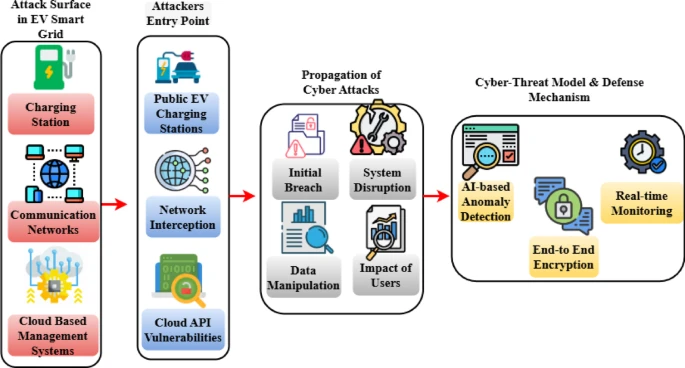
\includegraphics[width=0.7\textwidth]{pics/EVSE_attackpoints.png}
  \caption{EVSE as an access node to critical data\cite{nature2025}.}
  \label{fig:EVSE_attackpoints}
\end{figure}

With the access to these kind of Data the critical attacks like data manipulations, data theft, distrub of service up to complete system failure are possible\cite{nature2025}. That does not only comes with a high financial risk, it also affect the trust of the users in the EVSE systems and potentially slowing down the adoption of EVs in general.\\
If we provide end users with a stable and secure EVSE infrastructure, consumer confidence in switching to electric vehicles will be significantly higher. This, in turn, ensures a consistent growth in the adoption of both EVs and EVSE systems.

% https://papers.ssrn.com/sol3/papers.cfm?abstract_id=4768353 (Nutzervertrauen muss hergestellt werden)
% https://papers.ssrn.com/sol3/papers.cfm?abstract_id=4711137

\subsection{Challenges in securing EVSE infrastructure}

\subsection{Overview of AI-based approaches}

